\documentclass[12pt]{scrartcl}

\usepackage[utf8]{inputenc}
\usepackage[letterpaper]{geometry}
\usepackage{fancyhdr}
\usepackage{csquotes}
\usepackage[french]{babel}
\usepackage{graphicx}
\usepackage{minted}
\graphicspath{ {./images_rapport/} }

\pagestyle{fancy}
\fancyhead[R]{} % Active if we don't want the base fancy header
\fancyfoot[L]{INF1900}
\fancyfoot[R]{Librairies et débogage}

\author{Laurent Bourgon \\Mehdi Benouhoud \\Ihsane Majdoubi \\Catalina Andrea Araya Figueroa}
\subtitle{Travaux pratiques 7 et 8}
\title{Production de librairie statique et stratégie de débogage}

\date{Lundi 13 mars 2023}


\begin{document}
\maketitle



\newpage

\section{Description de la librairie}

\subsection{Classes}
\subsubsection{Led}
Depuis le début du cours, nous utilisons un diode électro-luminescente située
sur le circuit imprimé du robot. Cette diode est dite  \textquote{bi-colore}, c'est-à-dire
qu'elle peut s'allumer en rouge ou en vert, dépendament du sens du courant qu'on
lui transmets. En faisant clignoter rapidement la diode en alternant la couleur,
on obtient une troisième couleur: ambrée.

\begin{figure}[h]
    \centering
    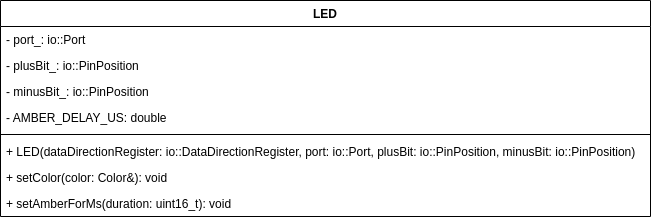
\includegraphics[scale=0.60]{LED_diagramme_classe}
    \caption{Diagramme de classe UML de \textbf{Led}}
\end{figure}

La classe est doté d'un constructeur, nous permettant d'indiquer où est branchée
la diode.
\begin{minted}{cpp}
    Led(io::DataDirectionRegister dataDirectionRegister, io::Port port,
        const io::PinPosition plus, const io::PinPosition minus)
\end{minted}

\mintinline{cpp}{dataDirectionRegister} indique le registre de direction des données où la
diode est branchée, \mintinline{cpp}{port} indique son port et finalement \mintinline{cpp}{plus}
et \mintinline{cpp}{minus} indique les broches sur lesquelles sont branchés la
respectivement cathode et l'anode de la diode. Il est important de respecter ce
sens afin de permettre à la méthode \mintinline{cpp}{setColor(const Color &color)} de
fonctionner adéquatement.
\\ \\
La méthode \mintinline{cpp}{setColor(const Color &color)} permet d'allumer la diode en rouge
ou en vert, en passant en paramètre \mintinline{cpp}{Color::RED} ou \mintinline{cpp}{Color::GREEN}.
\\ \\
La méthode \mintinline{cpp}{setAmberForMs(const uint16_t durationMs)} permets d'allumer la
diode en ambrée. Nous devont passer une durée (en milisecondes) en paramètre. En
effet, puisque la diode doit alterner rapidement entre le rouge et le vert, il
est impossible d'effectuer cette opération indéfiniement.
% TODO Peut-être mieux expliquer pourquoi on peut pas faire ça?
\newpage
\section{Modifications apportées au \textit{Makefile} de départ}
% Est-ce que je mets Makefile en « verb » ?
Depuis le début du cours, nous utilisons le \mintinline{cpp}{Makefile} fourni afin de
compiler notre code et l'installer sur le robot. Ayant créé une librairie, il a
fallu faire quelques modifications.
\subsection{Ajout d'une Makefile pour la librairie}
La compilation et l'archivage d'une librairie en un fichier \mintinline{cpp}{.a} implique
des variables et instructions supplémentaires par rapport à ce que le
\mintinline{cpp}{Makefile} de départ nous permettait de faire.

Ce nouveau \mintinline{cpp}{Makefile},
situé dans le répertoire \mintinline{cpp}{lib}, permets de faire l'édition et l'archivage
des liens des fichiers objets \mintinline{cpp}{.o} avec l'outil \mintinline{cpp}{avr-ar}. De plus il
contient quelques variables supplémentaires:
\begin{itemize}
    \item \verb|LIBNAME| qui indique le nom de la librairie (lib1900)
    \item \verb|SOURCES| et \verb|OBJECTS| qui indique les fichiers sources \verb|.cpp|
          et leurs fichiers objets homonymes en \verb|.o|
    \item \verb|ARTIFACTS| qui indique les fichiers artéfacts devant être supprimés
          dans le cas d'un \verb|make clean|
\end{itemize}
% Trouver moyen de faire un retour à la ligne
La librairie utilise des variables et règles communes à tous les \verb|Makefile|,
comme \verb|make clean|.

% Possiblement changer ce nom de section
\subsection{Encapsulation des variables et règles communes}
C'est pour cela que nous avons créé un \verb|Makefile.common|, situé à la racine
du dépôt afin qu'il puisse être importer partout, qui regroupe les éléments communs
aux \verb|Makefile|s de l'exécution et de la librairie.
\\ \\
Ce fichier regroupe notament les variables et la logique relié à
\begin{itemize}
    \item La supression d'artéfacts de compilation inutile, à l'aide de \verb|make clean|
    \item La compilation des fichiers sources \verb|.c| et \verb|.cpp| en fichiers
          objets \verb|.o|
    \item L'inclusion des fichiers de dépendances \verb|.d|
    \item La création d'archives binaires \verb|.hex| à partir des fichiers
          \verb|.elf|
    \item L'installation (ou \textit{flash}) du programme vers le
          microcontrôleur
\end{itemize}

Les deux \verb|Makefile|s peuvemt importer leurs éléments commun à l'aide de l'instruction

\begin{verbatim}
    include ../../../Makefile.common
\end{verbatim}

\subsection{Modifications au Makefile compilant le projet}
Outre les retraits de certaines variables et règles, qui sont désormais contenus
dans \verb|Makefile.common|, nous avons procédé à de petites modifications pour
que le compilateur inclut notre librairie lors de la compilation.

\end{document}